%!TEX root = informe.tex
\chapter{Proceso de fabricación, almacenaje, suministro y recepción}
Manual Euroadoquín. Documentos de Malaka.

\begin{figure}[!htb]
\centering
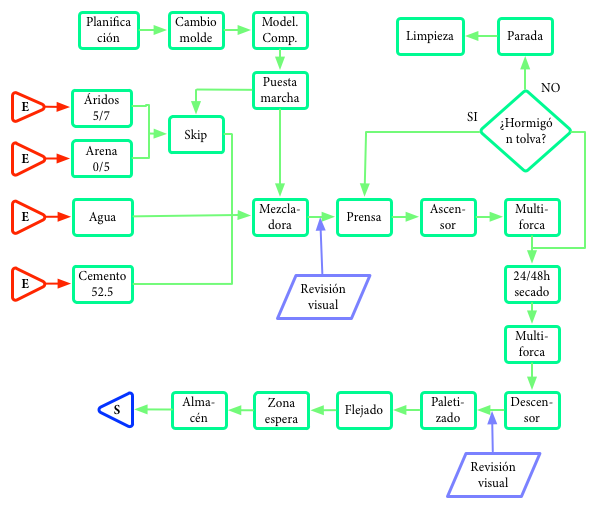
\includegraphics[width=15cm]{diagrama.png}
\caption{Diagrama de flujo de la fabricación de adoquines.}
\label{fig:diagrama_de_flujo}
\end{figure}

Cómo se construyen los bloques de adoquín

Las materias primas —cemento, arena, áridos y agua— se transportan hasta la planta de fabricación mediante camiones o ferrocarril. Actualmente los áridos y la arena ya no son apilados a bajo unos techados en las explanadas adyacentes a las plantas, sino que el propio transporte rellena las tolvas de forma automática.

Los áridos utilizados para producir adoquines puede incluir arena, gravilla y piedra de machaqueo si se pretende obtener un producto de peso normal. Si se desea que el adoquín sea más ligero —entre un 20 y un 45 \%— sin mermar sus propiedades estructurales se utilizan materiales como pizarra, arcilla, escoria de altos hornos y cenizas de carbón según su disponibilidad y coste.

Las tolvas tienen dosificadores que descargan la cantidad programada de materia prima sobre dos cintas transportadoras —una para áridos y arena, otra para cemento— con básculas de pesaje incorporadas que se comunican con el sistema de control y cortan el flujo de descarga.

La cinta de áridos descarga sobre un skip que eleva los materiales hasta una mezcladora. La cinta de cemento descarga directamente sobre la mezcladora.Previamente al añadido del agua se produce un ciclo de mezclado en seco. Para asegurar la consistencia del lote el agua es generalmente añadido mediante un sistema electrónico de control que dosifica el caudal. En el caso de que haya otros aditivos, tales como acelerantes o colorantes, es en este momento cuando se incorporan a la mezcla. Cuando se termina de añadir el agua se produce el mezclado creando hormigón fresco. El hormigón sale de la mezcladora mediante una cinta transportadora que contiene otra báscula de pesaje y se dirige hacia la tolva de hormigón que se encuentra en lo alto de la prensa, donde es dosificado en los moldes para adoquines. Los moldes tienen una longevidad muy alta —aproximadamente un millón de ciclos de prensado— y su durabilidad depende de las propiedades abrasivas de los áridos utilizados.

El molde se compone de dos partes: la parte donde se inyecta el hormigón (hembra) y la parte que se coloca encima para dar forma (macho). La prensa tiene incorporado un carro alimentador encargado de proporcionar la parte hembra. Se inyecta el hormigón en el molde hembra, el molde macho baja con la prensa y el hormigón es compactado y cimentado usando un sistema combinado de presión y vibración. Cada molde puede producir 25 adoquines de 200x100x60\si{\milli\meter}, lo que proporciona a una superficie adoquinada de 0.5\si{\square\meter}. Los adoquines son moldeados de una sola pieza y extraidos del molde inmediatamente después de la vibro-compresión sobre una bandeja de madera.

La bandeja con las piezas frescas es trasladada sobre un transportador de rodillos hasta un ascensor. Este ascensor tiene diez alturas, de forma que cada vez que recibe una bandeja con adoquines frescos, la bandeja anterior sube una altura y monta la siguiente.

El ascensor se encarga de alimentar un carro multiforca de diez alturas. Cuando las diez alturas está ocupadas se cargan en un carro multiforca automatizado que transporta las piezas hasta un secadero.

Las piezas permanecen en el secadero curándose a temperatura ambiente entre 24 y 48 horas.

Una vez transcurrido el tiempo de curado, los adoquines están secos y listos para ser recogidos por otro carro multiforca automatizado que recoge las bandejas y las lleva a un descensor.

El descensor coloca las bandejas con los adoquines secos en un transportador de rodillos.

El transportador de rodillos lleva las bandejas hasta una paletizadora para hacer bloques de hasta cinco alturas.

La paletizadora impulsa el pallet hasta la flejadora que aplica varias lazadas de flejes para evitar que los adoquines se desprendan del conjunto.

La flejadora descansa los conjuntos paletizados sobre un un transportador de rodillos para ser posteriormente llevados a almacén.

Finalmente, un torito transporta cada conjunto de adoquines a la zona de almacenaje.


\section{Dosificación}
\section{Amasado}
\section{Vibrocompresión}
\section{Curado}
\section{Embalaje y almacenamiento}
\section{Suministro}
\section{Recepción}
